\chapter[My Interaction with Prof. GR]{My Interaction with\\ Professor GR}

\Authorline{H K T Kumar}
\authinfo{Retd. Professor, Physics Department,\\ 
Siddaganga Institute of Technology, Tumkur}

I am Dr.\ H.\ K.\ T.\ Kumara, retired Professor in Physics Department, Siddaganga Institute of Technology, Tumakuru and I am very happy to share my personal interaction with Prof.\ G Ramachandran from 2011 to 2020. It was for the first time that I visited his house in Bengaluru on 2nd Feb 2011, after my M.Sc.\ (Batch of 1975) from Mysore University for an interaction with him. I wanted to request him to write a Text Book on Quantum Mechanics for Engineers basically for first year B.E. students. By definition we know that phase velocity $V_p=\omega/k$ and group velocity $V_g=d\omega/dk$.  My interest was in knowing whether there was a possibility of reduction of phase velocity from the relativistic expression for group velocity which I asked Prof.\ GR.\  He replied that it should be possible but I did not get the proof. Instead, he forwarded the eBook on Wave Propagation and Group velocity sent by Professor Mallesh.  He also made me to get the thesis of Yee Yee Oo through Dr.\ Vinay Deepak. Apart from this he had also sent the links to further readings on A new degree of freedom in Physics - Physics InSight 2/2011, Advances in Atomic Physics, Harmonic Analysis Method For Nonlinear Evolution Equations, Condensed Matter Physics, Nanoscience and Related Titles.  Also, he sent me a scientific article on the protein in human retina which may make it possible for mankind to have a ‘Sixth Sense’ after all: one that detects magnetic fields. This shows his generosity towards his students and he would go out of the way to help persons who had thirst for knowledge. 

Apart from his professional outlook, I had the unique opportunity to experience the human aspect of his personality.  He was very prompt and punctual in sending greetings to me, ever since my first visit to his home in 2011, on New Year, Sankranthi, Ugadi and Deepavali festivals.  His last greeting came in the New Year 2020.  Till this New Year I have never missed receiving greetings from him. I will always remember him for the cherished  moments spent with him and consider him as teacher amongst us forever. I take this opportunity to thank the family members of Prof.\ GR for their kind hospitality during my visit to his home.
\vskip 0.5cm

\centerline{\includegraphics[scale=1.3]{authorsphotos/Prof_H_K_T_Kumar.eps}}
\bigskip

\noindent
\textbf{Dr.\ H. K. T. Kumar} obtained the M.Sc.\ degree in 1975 from the Physics Department, Mysore University, and  Ph.D. from Bangalore University, in 1997. He joined the Physics Department, Siddaganga Institute of Technology, Tumkur, in 1976 and retired from there in 2014. Currently he leads an active retired life in Tumkur.
